\begin{flushright} {\tiny {\color{gray} \tt dlvsdlnro.tex}} \end{flushright}
%~~~~~~~~~~~~~~~~~~~~~~~~~~~~~~~~~~~~~~~~~~~~~~~~~~~~~~~~~~~~~~~~~~~~~~~~~~~

The mantle is heterogeneous but it is also inaccessible. This means that 
one must rely on indirect methods 
to probe its structure. Seismic tomography is a technique for imaging 
the subsurface of the Earth with seismic waves produced by earthquakes or explosions. 
P-, S-, and surface waves can be used for tomographic models of different resolutions.

Seismic velocity is a meaningful parameter for the interior dynamics of the
Earth because there exists a direct relation between seismic velocity and density. 
Such a relation was analysed experimentally by (for instance) Barton (1986) who 
used laboratory measurements of P-wave seismic velocity and density of rocks \cite{bart86}. 

Fourty years later or so, a crucial question remains: what is the exact form of the 
relation between density and seismic velocity for the entire Earth's mantle?

I will here not go into the details of the underlying theories and 
their approximations but will show a few useful results. 

From tomography to density, the workflow is usually as follows:
\[
d \ln V_p \rightarrow d \ln V_s \rightarrow d \ln \rho \rightarrow d\rho
\]
Note that if the method is based on shear wave tomography the conversion $d \ln V_p \rightarrow d \ln V_s$
is not necessary. 
Also the last step $d \ln \rho \rightarrow d\rho$ requires a background density field, 
often taken to be either the PREM model or AK135 (see Section~\ref{ss:prem}). 

On the following plots are shown radial averages of the 
ratio $d \ln V_s/d\ln V_p$ and/or $d\ln \rho/d \ln V_s$:

\begin{center}
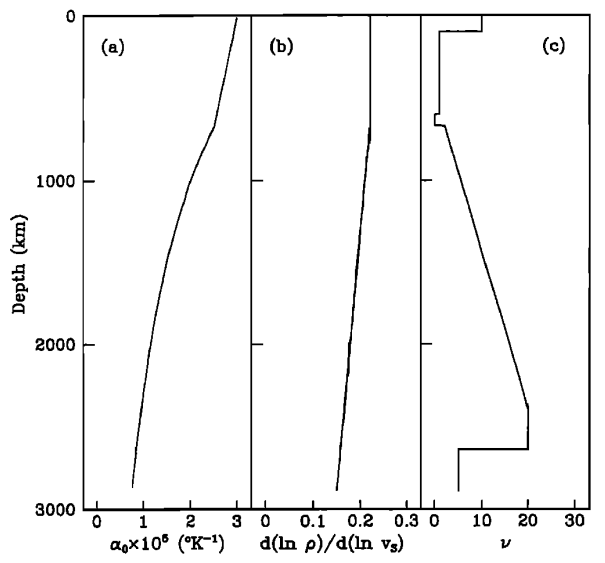
\includegraphics[width=7cm]{images/thermal_expansion/pape95}\\
{\captionfont Taken from \textcite{pape95} (1995).}
\end{center}

\begin{center}
\includegraphics[height=5cm]{images/dlnvsdlnrho/moek16b}
\includegraphics[height=5cm]{images/dlnvsdlnrho/moek16a}\\
{\captionfont Taken from Moulik \& Ekstrom (2016) \cite{moek16}}
\end{center}

\begin{center}
\includegraphics[height=6cm]{images/dlnvsdlnrho/xi.pdf}\\
{\captionfont Profiles of scaling factor $\xi=d \ln \rho/d\ln V_s$. Data from 
Steinberger \& Calderwood (2006) \cite{stca06} and Moulik \& Ekstrom (2016) \cite{moek16}.
Data available in images/dlnrhodlnvs/} 
\end{center}

Then
\[
\delta \ln(\rho(r,\theta,\phi)) = \xi(r) \cdot \delta \ln (V_s(r,\theta,\phi) )
\]
with  
\[
\delta \ln (\rho(r,\theta,\phi)) = \frac{ \delta \rho(r,\theta,\phi)}{\rho_{ref}(r)}
\]
where $\rho_{ref}$ is a radial profile, PREM for instance in the case of S40RTS 
so finally 
\[
\delta \rho(r,\theta,\phi) 
= \rho_{ref}(r) \cdot  \delta \ln(\rho(r,\theta,\phi)) 
= \rho_{ref}(r)\cdot \xi(r) \cdot \delta \ln(V_s(r,\theta,\phi)) 
\]






\Literature: \cite{roma01}
